\chapter{Firme Digitali}
Una firma digitale è l'equivalente informatico di una tipica firma convenzionale. La struttura è molto simile a quella del Message Authentication, tuttavia qui abbiamo una struttura simmetrica in cui abbiamo una chiave segreta che serve a firmare e una chiave pubblica che serve per verificare. 
Una firma digitale deve garantire \textbf{non ripudiabilità} e questo è garantito dal fatto che la natura asimmetrica di questa procedura, fa sì che solo l'utente che possiede la chiave privata possa firmare. Uno schema di firma digitale è formato dai seguenti algoritmi:
\begin{itemize}
    \item Algoritmo di generazione della chiave: che è un algoritmo randomizzato che restituisce una coppia \textbf{(vk, sk)} dove vk è la chiave di verifica, mentre sk è la chiave di firma.
    \item Algoritmo di firma: algoritmo che prende in input sk e un messaggio m e restituisce una firma $\sigma$ o un simbolo di errore.
    \item Algoritmo di verifica: algoritmo deterministico che prende in input vk, m e $\sigma$ e restituisce 1 se la firma è valida, 0 altrimenti.
\end{itemize}

Definiamo la sicurezza di uno schema di firma in maniera simile a quanto già fatto per quanto riguarda MA:
\begin{figure}[H]
    \centering
    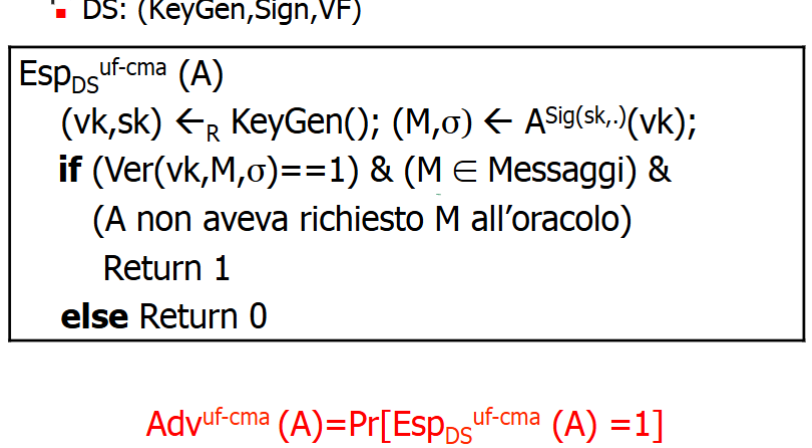
\includegraphics[width=0.6\linewidth]{Images/firma_digitale/sicurezza_ds.png}
\end{figure} 
In questo caso non abbiamo più bisogno di un oracolo di verifica come accadeva per il MAC poiché abbiamo che la chiave di verifica è pubblica. 
\section{Firma RSA}
L'idea alla base di questo sistema di firma è quello di sfruttare la funzione trapdoor in modo inverso a quanto fatto precedentemente per cifrare. Nel caso di RSA:
\begin{itemize}
    \item L'algoritmo di cifratura diventa l’algoritmo di verifica.
    \item L'algoritmo di decifratura diventa l’algoritmo di firma.
    \item L'algoritmo di generazione delle chiavi resta invariato.
\end{itemize}
Vediamo precisamente gli algoritmi:
\begin{figure}[H]
    \centering
    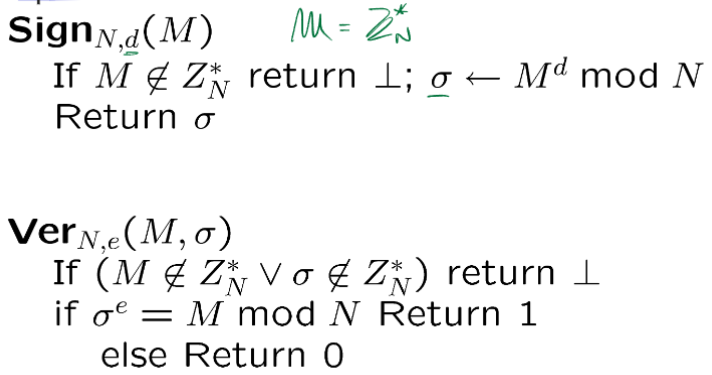
\includegraphics[width=0.6\linewidth]{Images/firma_digitale/sign_ver_rsa.png}
\end{figure} 
Purtroppo, a causa della natura di cifratura di RSA, se N è di 3000 bit, posso cifrare solo messaggi di 3000 bit e ciò lo rende poco usabile. Inoltre, lo schema non è sicuro poiché $Ver(1,1)$ è sempre vero senza nemmeno dover chiedere mai nulla all'oracolo di firma. 
Inoltre, poiché $e$ è pubblico\footnote{$e$ è pubblico poiché è la chiave di verifica}, è possibile generare firme casuali ed elevarli a $e$ per avere una coppia valida. E si può anche dimostrare l'esistenza di un altro attacco che permette la cifratura di messaggi arbitrari. Li vediamo in figura entrambi gli attaccanti rispettivamente come A e B.
\begin{figure}[H]
    \centering
    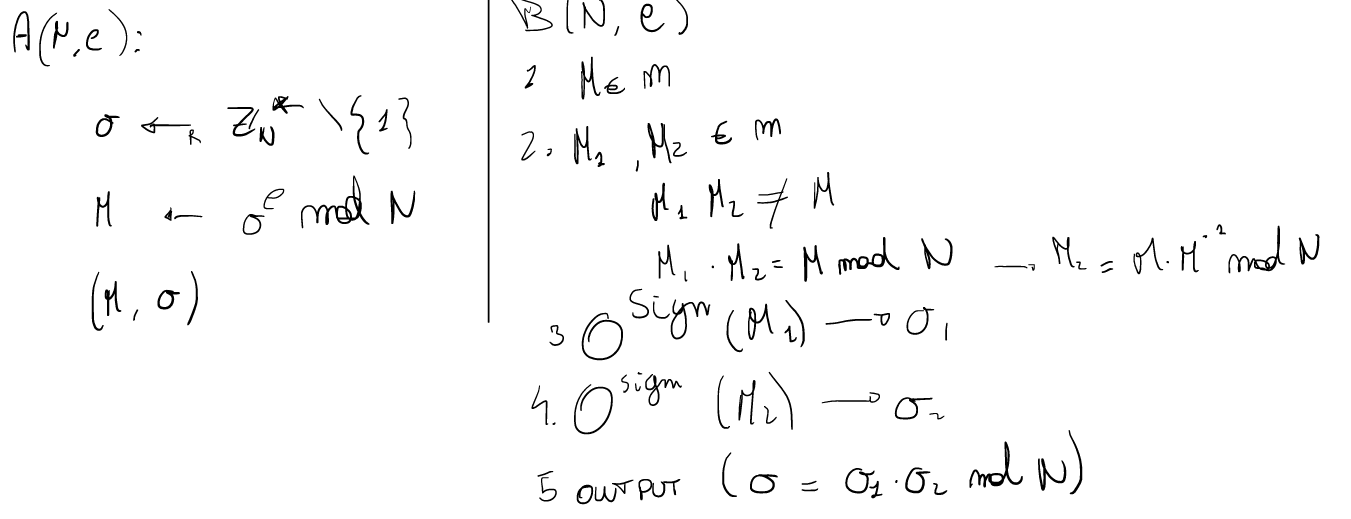
\includegraphics[width=0.7\linewidth]{Images/firma_digitale/attacco_firma_rsa.png}
\end{figure} 

\section{Approccio Hash e Inverti}
Ci serve un modo per far sì che M sia una stringa arbitraria e per "distruggere" le proprietà algebriche di RSA. Per fare ciò, ci basta utilizzare una funzione Hash come segue:
\begin{figure}[H]
    \centering
    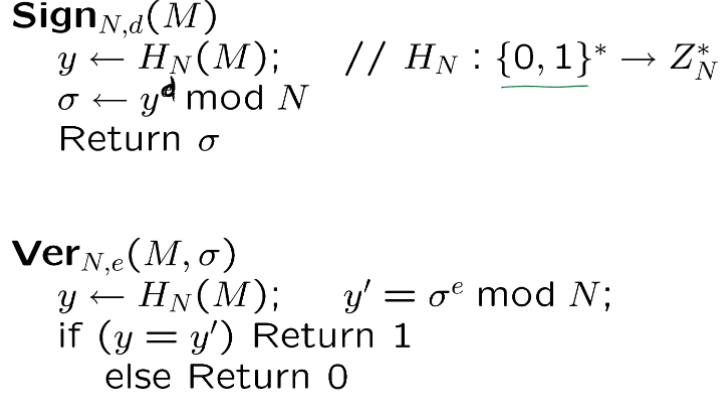
\includegraphics[width=0.7\linewidth]{Images/firma_digitale/hash_inverti.png}
\end{figure} 
Dove H è resistente alle collisioni, intrattabile da invertire e che possa prendere messaggi arbitrari. Per verificare la sicurezza nel caso di Hash e inverti, ci mettiamo nuovamente nel contesto di Random Oracle, per cui:
\begin{figure}[H]
    \centering
    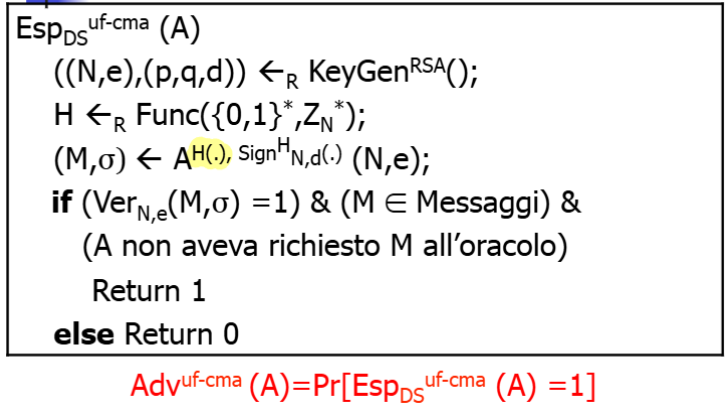
\includegraphics[width=0.7\linewidth]{Images/firma_digitale/sicurezza_uf_cma_ds.png}
\end{figure} 
Come possiamo vedere, A adesso ha la necessità di avere un oracolo di Hash poiché l'hash è un random oracle.

Un teorema ci dice che: Sia A un avversario che fa al più $q_s$ richieste di firma e $q_h$ richieste all'oracolo di Hash. Esiste un avversario $I$ che usa risorse comparabili ad A tale che:
\[Adv^{uf-cma}(A)\leq q_h \quad Adv^{ow-rsa}(I)\]
Dove $q_h$ non è trascurabile. Per cui, questo fa' sì che abbiamo bisogno di un modulo RSA abbastanza grande da rendere $q_h$ trascurabile. Tuttavia, maggiore è il modulo RSA, meno è scalabile, dunque, non potendo ignorare $q_h$, si passa a schemi randomizzati.
\section{EC-DSA e Schorr's Signature}
Vediamo in breve questo schema:
\begin{figure}[H]
    \centering
    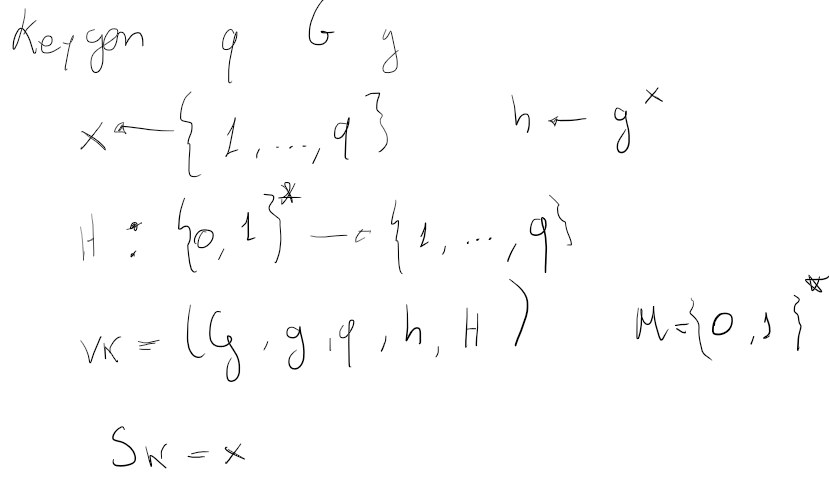
\includegraphics[width=0.7\linewidth]{Images/firma_digitale/ec_dsa_key_gen.png}
\end{figure} 
\begin{figure}[H]
    \centering
    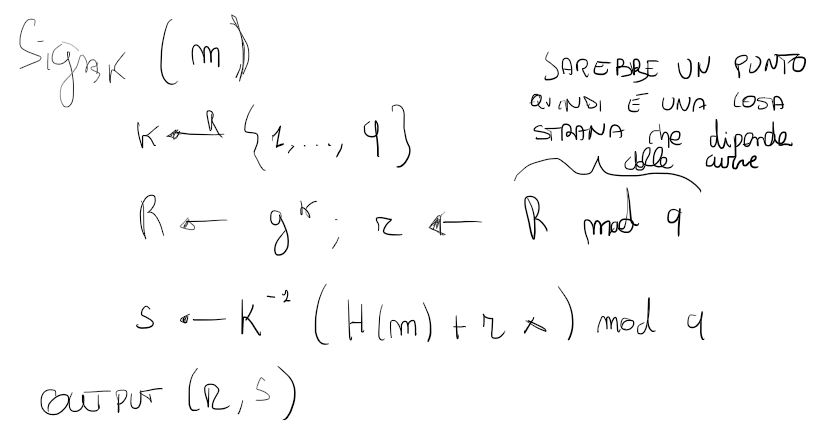
\includegraphics[width=0.7\linewidth]{Images/firma_digitale/ec_dsa_sign.png}
\end{figure} 
\begin{figure}[H]
    \centering
    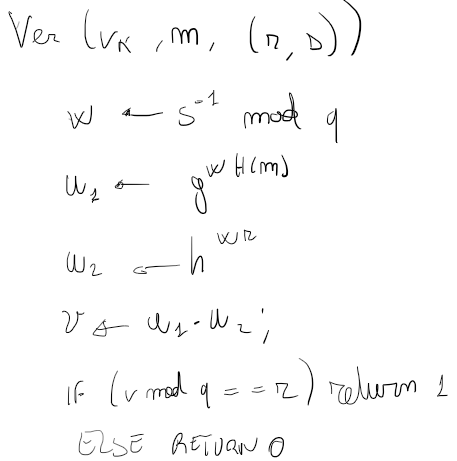
\includegraphics[width=0.5\linewidth]{Images/firma_digitale/ec_dsa_ver.png}
\end{figure} 
\begin{figure}[H]
    \centering
    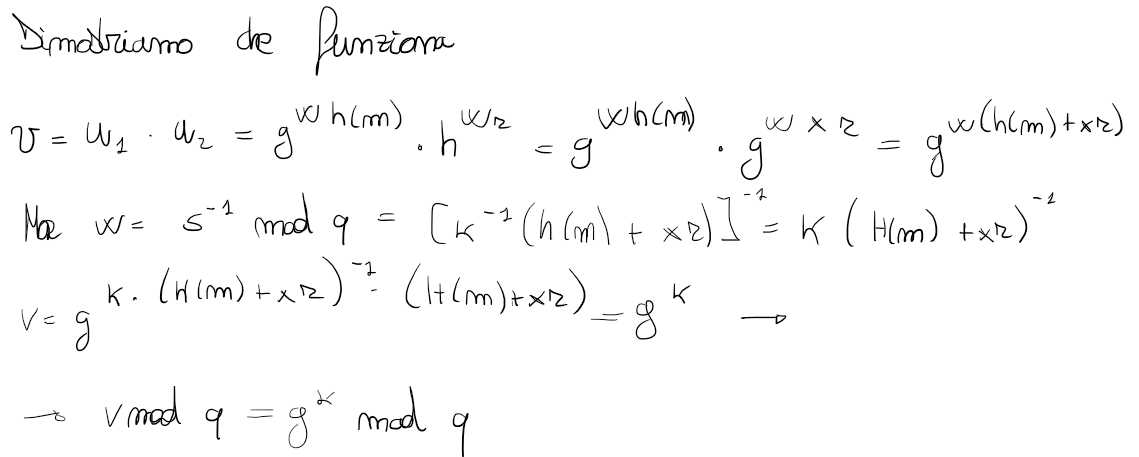
\includegraphics[width=0.8\linewidth]{Images/firma_digitale/ec_dsa_correttezza.png}
\end{figure} 
Per quanto riguarda, invece, il sistema di \textbf{Schorr's Signature} abbiamo che:
\begin{figure}[H]
    \centering
    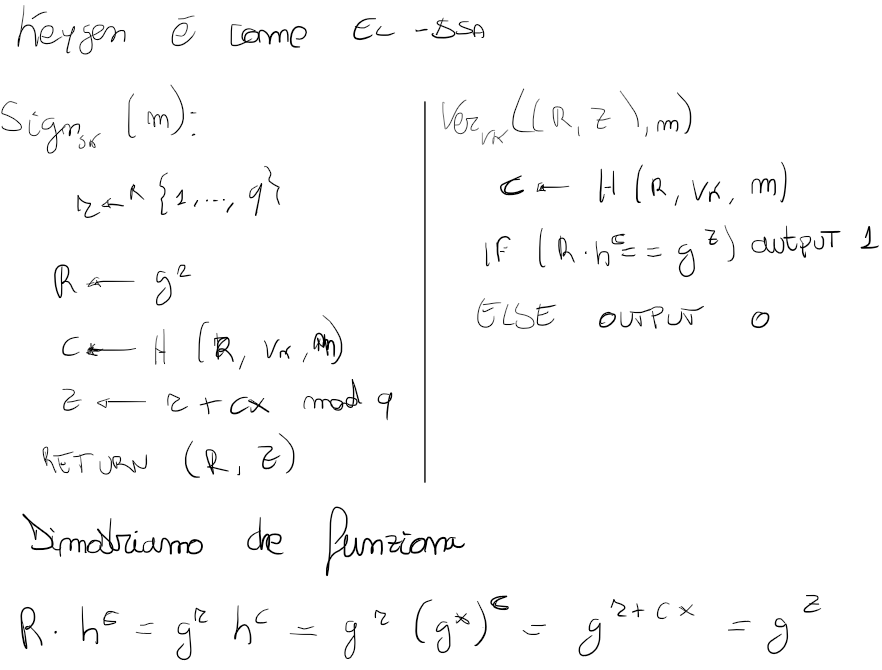
\includegraphics[width=0.8\linewidth]{Images/firma_digitale/schors_signature.png}
\end{figure} 